
\title[Control of Line Pack in Natural Gas System of Israel]{Control of Line Pack in Natural Gas System of Israel:
Balancing Limited Resources under Uncertainty}
\author[Hyett, Pagnier, Alisse, Saban, Goldshtein, Chertkov]{Criston Hyett, Laurent Pagnier, Jean Alisse, Lilah Saban, Igal Goldshtein, Misha Chertkov}

\institute{The University of Arizona \& NOGA Israel}

\graphicspath{{./NOGA-UA-gas/figs/}}
% -------------------------------------------------------------------------------%
\begin{frame}
  \maketitle
\end{frame}
% -------------------------------------------------------------------------------%
% -------------------------------------------------------------------------------%
\begin{frame}{Context}
  \begin{columns}
    \begin{column}{0.5\textwidth}
      \begin{figure}
        \centering
        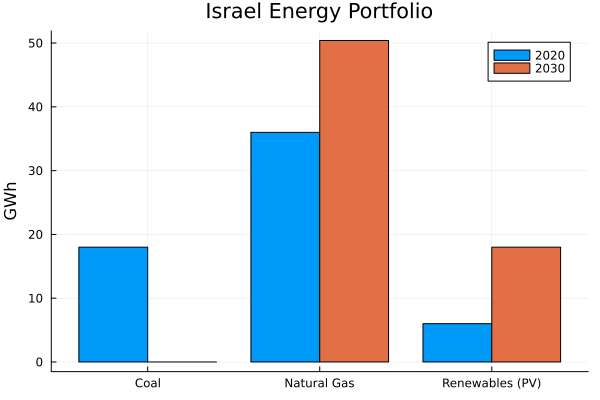
\includegraphics[width=\textwidth]{energyPortfolio.png}
      \end{figure}
    \end{column}

    \begin{column}{0.5\textwidth}
      \begin{figure}
        \centering
        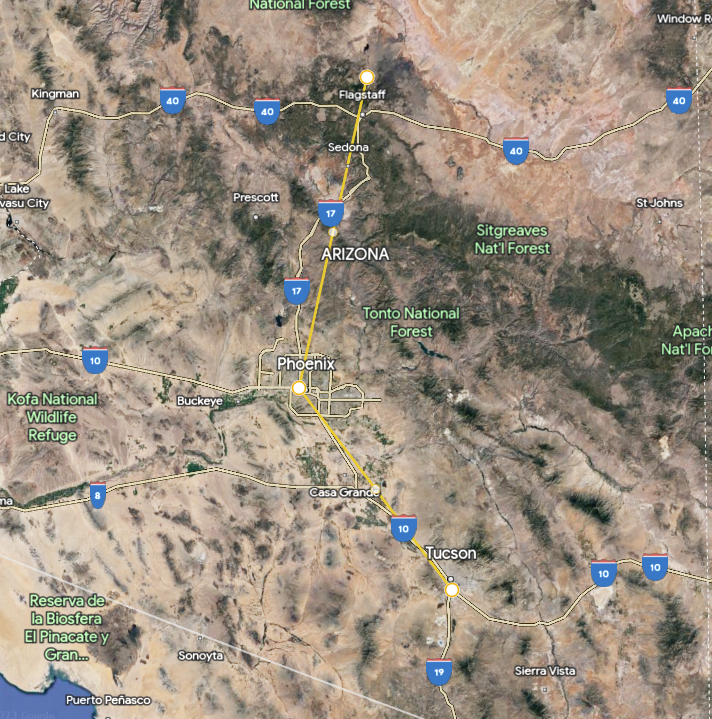
\includegraphics[width=0.75\textwidth]{israelLengthOnAZ.png}
      \end{figure}
    \end{column}
  \end{columns}
\end{frame}
% -------------------------------------------------------------------------------%

% -------------------------------------------------------------------------------%
\begin{frame}{Project Goals}
  \begin{itemize}
  \item Operations-aware modeling and simulation of a reduced model of Israel's natural gas network.
    \begin{itemize}
    \item Flux control at inlet nodes
    \item Realistic initial conditions
    \item Assessing relevant challenges
      \begin{itemize}
      \item Robustness in the case of uncertain PV generation
      \item Robustness in the case of an insult to the system
      \end{itemize}
    \end{itemize}

  \item Model \& open-source tool development
    \begin{itemize}
    \item Solver suite specifically suited to the needs of natural gas networks
    \item Advanced automatic controls
    \item Monte-Carlo/Uncertainty Quantification
    \end{itemize}
  \end{itemize}
\end{frame}
% -------------------------------------------------------------------------------%

% -------------------------------------------------------------------------------%
\begin{frame}{Reduced Model of Israel's Gas Network}
  \begin{center}
    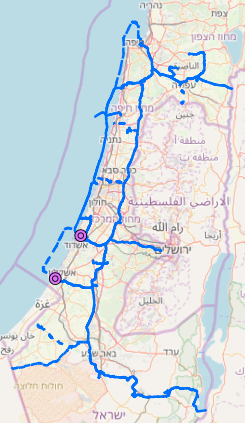
\includegraphics[width=0.25\textwidth]{fullModel.png}
    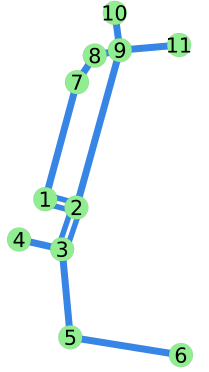
\includegraphics[width=0.25\textwidth]{reducedModel.png}
  \end{center}
  \footnotetext{\url{https://www.gov.il/he/departments/guides/distribution_area}}
\end{frame}
% -------------------------------------------------------------------------------%

% -------------------------------------------------------------------------------%
\begin{frame}{Effective Gas Flow Equations}
  Under reasonable assumptions, the system of PDEs governing gas flow is 
  \begin{align}
    \partial_t \rho & + \partial_x \phi = 0\\
    \partial_t \phi & + \partial_x P = -\beta \frac{\phi|\phi|}{\rho}
  \end{align}
  These, supplemented with initial
  \begin{align}
    \rho(x,0) &= \rho_0(x)\\
    \phi(x,0) &= \phi_0(x)
  \end{align}
  and boundary conditions at each node
  \begin{equation}
    \rho_i(t) \text{ \emph{or} } \phi_i(t)
  \end{equation}
  and an equation of state relating pressure and density
  \begin{equation}
    P(\rho) = ... \quad \rho(P) = ...
  \end{equation}
\end{frame}
% -------------------------------------------------------------------------------%

% -------------------------------------------------------------------------------%
\begin{frame}{Staggered Grid Method}
  \begin{columns}
    \begin{column}{0.6\textwidth}
      \begin{figure}
        \centering
        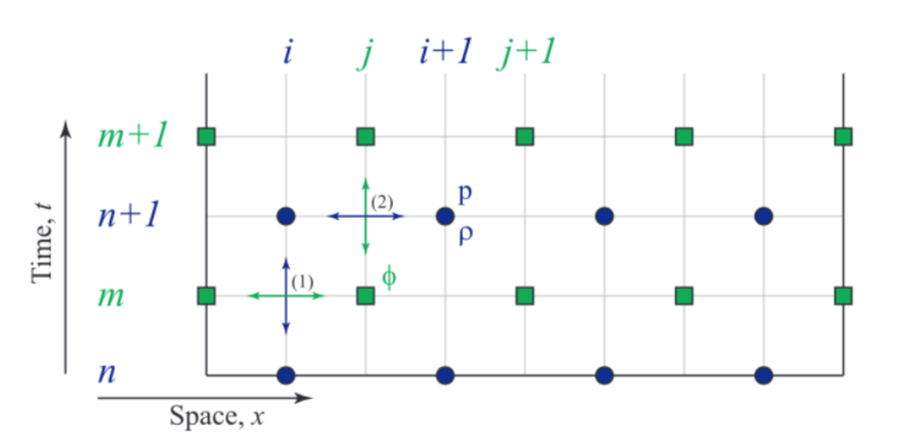
\includegraphics[width=1.0\textwidth]{ScenarioResults/staggeredGrid.png}
        \caption{Figure taken from Gyrya,Zlotnik: "An explicit staggered-grid method for numerical simulation of large-scale natural gas pipeline networks"}
        \label{fig:my_label}
      \end{figure}
    \end{column}

    \begin{column}{0.4\textwidth}
      \begin{equation*}
        \color{blue} \partial_t \rho + \partial_x \phi = 0
      \end{equation*}
      \begin{equation*}
        \color{ForestGreen} \partial_t \phi + \partial_x P = -\beta \frac{\phi|\phi|}{\rho}
      \end{equation*}
      CFL stability condition:
      \begin{equation*}
        \sqrt{P'(\rho)} \frac{\Delta t}{\Delta x} \leq 1
      \end{equation*}
    \end{column}
  \end{columns}
\end{frame}
% -------------------------------------------------------------------------------%

% -------------------------------------------------------------------------------%
\begin{frame}{Results: Scenario 1}
  \begin{figure}
    \centering
    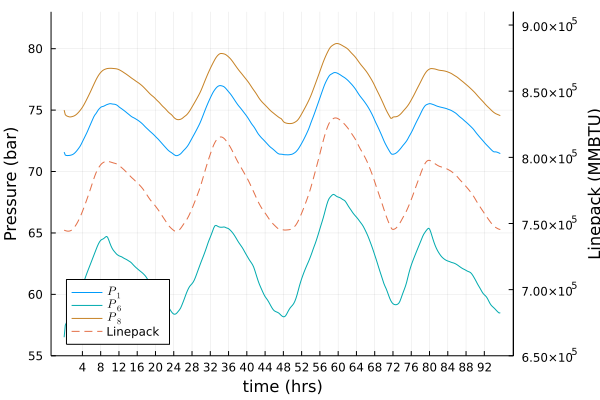
\includegraphics[width=0.65\textwidth]{ScenarioResults/scen1.png}
    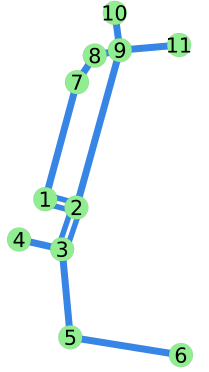
\includegraphics[width=0.25\textwidth]{reducedModel.png}
    \caption{Nominal week in August.}
  \end{figure}
\end{frame}
% -------------------------------------------------------------------------------%

% -------------------------------------------------------------------------------%
\begin{frame}{Uncertainty}
  Moderate uncertainty at demand nodes is represented through addition of a random noise at the consumption site
  \begin{equation}
    d_i(t) \to X_i(t)
  \end{equation}
  where
  \begin{equation}
    dX_i(t) = \alpha(d_i(t) - X_i(t))dt + \gamma dW
  \end{equation}
  is a Ornstein–Uhlenbeck process
  \begin{itemize}
  \item $\mathbb{E}[X_i(t)] = d_i(t)$
    \vspace{0.1cm}
  \item $ \text{Var}(X_i(t)) = \frac{\gamma}{2\alpha}\left(1 - e^{-2\alpha t} \right) $
    \vspace{0.1cm}
  \item The parameters were tuned heuristically to ensure the mean was respected, and the variance approaches
    \begin{equation}
      \text{Var}(X_i(t)) \approx 0.01 \mu_i^2
    \end{equation}
    With $\mu_i$ being the mean withdrawal of node $i$.
  \end{itemize}

\end{frame}
% -------------------------------------------------------------------------------%


% -------------------------------------------------------------------------------%
\begin{frame}{Results: Scenario 2}
  \begin{figure}
    \centering
    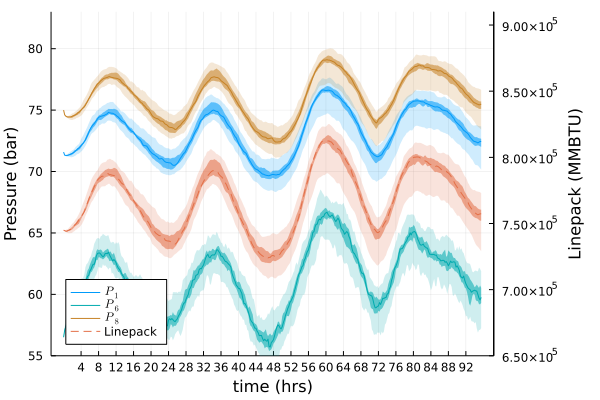
\includegraphics[width=0.65\textwidth]{ScenarioResults/scen2.png}
    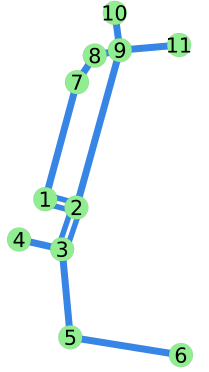
\includegraphics[width=0.25\textwidth]{reducedModel.png}
    \caption{Linepack and pressures for random perturbation on top of nominal August days.}
  \end{figure}
\end{frame}
% -------------------------------------------------------------------------------%

% -------------------------------------------------------------------------------%
\begin{frame}{Results: Scenario 3 \& 4}
  \begin{figure}
    \centering
    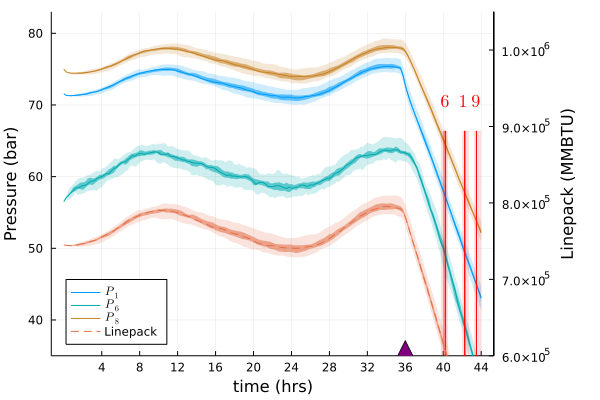
\includegraphics[width=0.45\textwidth]{ScenarioResults/scen3.png}\hspace{0.6cm}%
    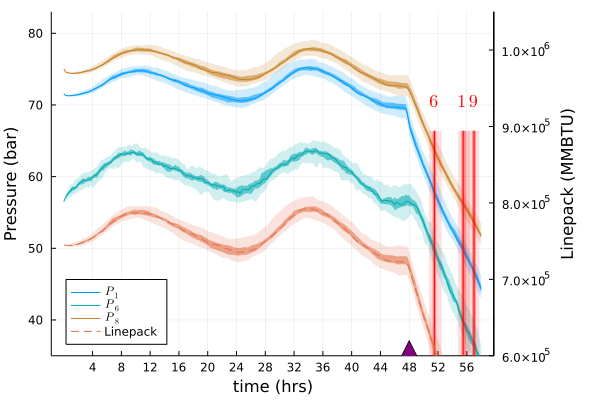
\includegraphics[width=0.45\textwidth]{ScenarioResults/scen4.png}
    \caption{Linepack and pressures responding to loss of supply at node 1. (Left) shows the insult at a peak of intraday linepack, and (right) shows the same insult at the trough.}
  \end{figure}
  \begin{columns}
    \begin{column}{0.5\textwidth}
      \begin{equation*}
        \tau = 4.13 \pm 0.38 \text{ hrs}
      \end{equation*}
    \end{column}

    \begin{column}{0.5\textwidth}
      \begin{equation*}
        \tau = 3.58 \pm 0.89 \text{ hrs}
      \end{equation*}
    \end{column}
  \end{columns}
\end{frame}
% -------------------------------------------------------------------------------%


% -------------------------------------------------------------------------------%
\begin{frame}{Results: Scenario 5}
  \begin{figure}
    \centering
    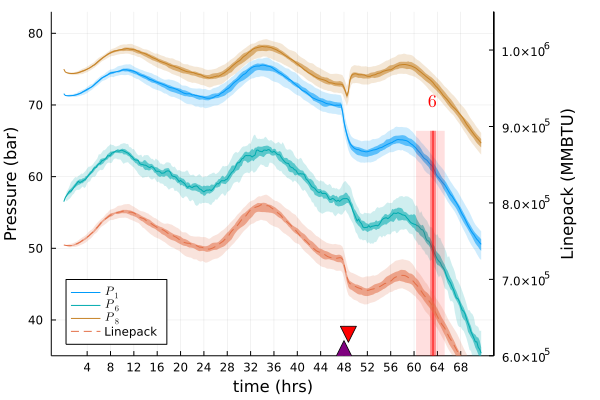
\includegraphics[width=0.65\textwidth]{ScenarioResults/scen5.png}
    \caption{Linepack and pressures for insult at hour 48, implementing a max-flow control on the remaining supply at node 8. $\tau = 14.17 \pm 4.07 \text{ hrs}$}
  \end{figure}
\end{frame}
% -------------------------------------------------------------------------------%

% -------------------------------------------------------------------------------%
\begin{frame}{Results: Scenario 6}
  \begin{figure}
    \centering
    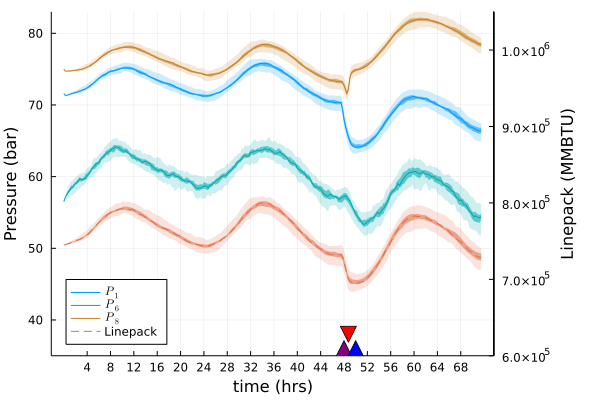
\includegraphics[width=0.65\textwidth]{ScenarioResults/scen6.png}
    \caption{Linepack and pressures for insult at hour 48, implementing a max-flow control on the remaining supply at node 8, and curtailing demand 2 hours after the insult.}
  \end{figure}
\end{frame}
% -------------------------------------------------------------------------------%

%-------------------------------------------------------------------------------%
\begin{frame}{Next Steps}
  \begin{itemize}
  \item Better UQ: Stochastic Finite Volumes(?)
  \item Higher order method and efficient implementation to allow for parallelization and acceleration.
  \item Advanced automatic controls
    \begin{itemize}
    \item This would mimick some actual protocol, and allow you to make statements such as, "with 95\% confidence, using protocol A, the natural gas system is robust to an insult of type B"
    \end{itemize}
  \item Simulation and optimization of the joint power and gas grids, under uncertainty.
  \end{itemize}
\end{frame}
%-------------------------------------------------------------------------------%

%-------------------------------------------------------------------------------%
\begin{frame}{Questions/Comments/Suggestions?}
  \begin{itemize}
  \item cmhyett@math.arizona.edu
  \item \url{https://arxiv.org/abs/2304.01955}
  \item \url{https://github.com/cmhyett/FluxControlLinepack}
  \end{itemize}  
\end{frame}
% -------------------------------------------------------------------------------%